\chapter{Lattice Element Types}
\label{c:ele.types}

%---------------------------------------------------------------------------------------------------

This chapter discusses the various types of elements
available in \accellat.
These elements are:
\begin{table}[htb]
\centering
{\tt
\begin{tabular}{llll} \toprule
  {\it Element}     & {\it Section}         & {\it Element}      & {\it Section}      \\ \midrule
  ACKicker          & \ref{s:ackicker}      &  Marker           & \ref{s:marker}      \\
  BeamBeam          & \ref{s:beambeam}      &  Mask             & \ref{s:mask}        \\
  BeginningEle      & \ref{s:begin.ele}     &  Match            & \ref{s:match}       \\
  Bend              & \ref{s:bend}          &  Multipole        & \ref{s:mult}        \\
  Converter         & \ref{s:converter}     &  NullEle          & \ref{s:nullele}     \\
  Collimator        & \ref{s:collimator}    &  Octupole         & \ref{s:octupole}    \\
  CrabCavity        & \ref{s:crabcavity}    &  Patch            & \ref{s:patch}       \\
  Drift             & \ref{s:drift}         &  Quadrupole       & \ref{s:quadrupole}  \\
  EGun              & \ref{s:egun}          &  RFCavity         & \ref{s:rfcavity}    \\
  Fiducial          & \ref{s:fiducial}      &  Sextupole        & \ref{s:sextupole}   \\
  FloorShift        & \ref{s:floorshift}    &  Solenoid         & \ref{s:solenoid}    \\
  Foil              & \ref{s:foil}          &  Taylor           & \ref{s:taylor}      \\
  Fork              & \ref{s:fork}          &  ThickMultipole   & \ref{s:thickmult}   \\
  Girder            & \ref{s:girder}        &  Undulator        & \ref{s:undulator}   \\
  Instrument        & \ref{s:instrument}    &  UnionEle         & \ref{s:unionele}    \\
  Kicker            & \ref{s:kicker}        &  Wiggler          & \ref{s:wiggler}     \\
  LCavity           & \ref{s:lcavity}       &                   &                     \\
  \bottomrule
\end{tabular}
} 
\caption{Table of element types.}
\label{t:particle.classes}
\end{table}

\newpage

%---------------------------------------------------------------------------------------------------
\section{ACKicker}
\label{s:ackicker}

An \vn{ac_kicker} element simulates a ``slow'' time dependent kicker element.

NOTE: This Element is in development and is incomplete. 
Missing: Need to document amp_function function to return the kick amplitude.

Element parameter groups associated with this element type are:
\TOPrule 
\begin{example}
  AlignmentGroup     -> Element position/orientation shift. \sref{s:align.g} 
  ApertureGroup      -> Vacuum chamber aperture. \sref{s:aperture.g} 
  BMultipoleGroup    -> Magnetic multipoles. \sref{s:bmultipole.g} 
  FloorPositionGroup -> Global floor position and orientation. \sref{s:floor.pos.g} 
  LengthGroup        -> Length and s-position parameters. \sref{s:length.g} 
  LordSlaveGroup     -> Element lord and slave status. \sref{s:lord.slave.g} 
  MasterGroup        -> Contains field_master parameter. \sref{s:master.g} 
  ReferenceGroup     -> Reference energy and species. \sref{s:reference.g} 
  DescriptionGroup   -> Element descriptive strings. \sref{s:descrip.g} 
  TrackingGroup      -> Default tracking settings. \sref{s:tracking.g} 
\end{example}
\BOTTOMrule


The calculated field will only obey Maxwell's equations in the limit that the time variation
of the field is ``slow'':
\begin{equation}
  \omega \ll \frac{c}{r}
\end{equation}
where $\omega$ is the characteristic frequency of the field variation, $c$ is the speed of light,
and $r$ is the characteristic size of the \vn{ACKicker} element. That is, the fields at opposite
ends of the element must be able to ``communicate'' (which happens at the speed of light) in a time
scale short compared to the time scale of the change in the field.

\newpage

%---------------------------------------------------------------------------------------------------
\section{BeamBeam}
\label{s:beambeam}

A \vn{beambeam} element simulates an interaction with an opposing
(``strong'') beam traveling in the opposite direction.

NOTE: This Element is in development and is incomplete

Element parameter groups associated with this element type are:
\TOPrule
\begin{example}
  FloorPositionGroup -> Global floor position and orientation. \sref{s:floor.pos.g} 
  LengthGroup        -> Length and s-position parameters. \sref{s:length.g} 
  LordSlaveGroup     -> Element lord and slave status. \sref{s:lord.slave.g} 
  ReferenceGroup     -> Reference energy and species. \sref{s:reference.g} 
  DescriptionGroup   -> Element descriptive strings. \sref{s:descrip.g} 
  TrackingGroup      -> Default tracking settings. \sref{s:tracking.g} 
\end{example}
\BOTTOMrule


\newpage

%---------------------------------------------------------------------------------------------------
\section{BeginningEle}
\label{s:begin.ele}

A \vn{BeginningEle} element must be present as the first element of every tracking branch.
(\sref{s:branch.def}).

Element parameter groups associated with this element type are:
\TOPrule
\begin{example}
  FloorPositionGroup -> Global floor position and orientation. \sref{s:floor.pos.g} 
  InitParticleGroup  -> Initial particle position and spin. \sref{s:init.particle.g} 
  LengthGroup        -> Length and s-position parameters. \sref{s:length.g} 
  LordSlaveGroup     -> Element lord and slave status. \sref{s:lord.slave.g} 
  ReferenceGroup     -> Reference energy and species. \sref{s:reference.g} 
  DescriptionGroup   -> Element descriptive strings. \sref{s:descrip.g} 
  TrackingGroup      -> Default tracking settings. \sref{s:tracking.g} 
  TwissGroup         -> Initial Twiss and coupling parameters. \sref{s:twiss.g} 
\end{example}
\BOTTOMrule


Example:
\begin{example}
  @ele bg = BeginningEle(species_ref = Species("proton"), pc_ref = 1e11)
\end{example}

\newpage

%---------------------------------------------------------------------------------------------------
\section{Bend}
\label{s:bend}

A \vn{Bend} element represents a dipole bend. Bends have a design bend angle and bend radius
which determines the location of downstream elements as documented in \sref{s:machine.coords}.
The actual bending strength that a particle feels can differ from the design value as detailed
below.

Element parameter groups associated with this element type are:
\TOPrule
\begin{example}
  AlignmentGroup     -> Element position/orientation shift. \sref{s:align.g} 
  ApertureGroup      -> Vacuum chamber aperture. \sref{s:aperture.g} 
  BMultipoleGroup    -> Magnetic multipoles. \sref{s:bmultipole.g} 
  BendGroup          -> Bend element parameters. \sref{s:bend.g} 
  EMultipoleGroup    -> Electric multipoles. \sref{s:emultipole.g} 
  FloorPositionGroup -> Global floor position and orientation. \sref{s:floor.pos.g} 
  LengthGroup        -> Length and s-position parameters. \sref{s:length.g} 
  LordSlaveGroup     -> Element lord and slave status. \sref{s:lord.slave.g} 
  MasterGroup        -> Contains field_master parameter. \sref{s:master.g} 
  ReferenceGroup     -> Reference energy and species. \sref{s:reference.g} 
  DescriptionGroup   -> Element descriptive strings. \sref{s:descrip.g} 
  TrackingGroup      -> Default tracking settings. \sref{s:tracking.g} 
\end{example}
\BOTTOMrule


\begin{figure}[ht]
  \centering 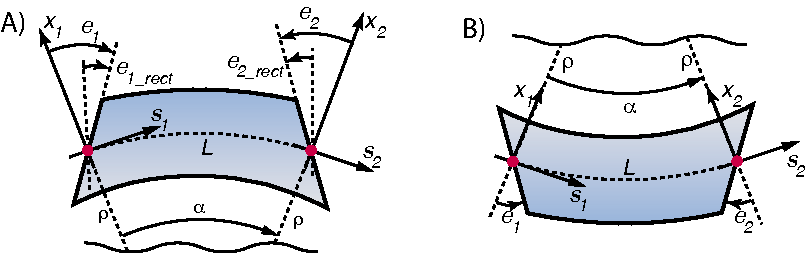
\includegraphics{bend.pdf} 
\caption[Bend geometry]{
Bend geometry. Red dots are the entry and exit points that define the origin for the
coordinate systems at the entry end $(s_1, x_1)$ and exit ends $(s_2, x_2)$ respectively. 
In the figure, the angle \vn{alpha} is denoted $\alpha$ and the radius
\vn{rho} is denoted $\rho$.
A) Bend geometry with positive bend angle. For the geometry shown, 
\vn{g}, \vn{angle}, \vn{rho}, \vn{e1}, \vn{e2}, \vn{e1_rect}, and \vn{e2_rect} are all positive.
B) Bend geometry with negative bend angle. For the geometry shown, 
\vn{g}, \vn{angle}, \vn{rho}, \vn{e1}, \vn{e2}, \vn{e1_rect}, and \vn{e2_rect} are all negative.
Note: The figures are drawn for zero \vn{ref_tilt} where the rotation axis is parallel to the 
$y$-axis. 
}
\label{f:bend2}
\end{figure}

The \vn{BendGroup} group (\sref{s:bend.g}) contains the parameters that define the shape of the bend.

Example:
\begin{example}
  @ele b03w = Bend(l = 0.6, g = 0.017, kn1 = 0.003)
\end{example}

\newpage

%---------------------------------------------------------------------------------------------------
\section{Collimator}
\label{s:collimator}

\vn{Collimators} are field free elements that can collimate beam particles.

Element parameter groups associated with this element type are:
\TOPrule
\begin{example}
  FloorPositionGroup -> Global floor position and orientation. \sref{s:floor.pos.g} 
  LengthGroup        -> Length and s-position parameters. \sref{s:length.g} 
  LordSlaveGroup     -> Element lord and slave status. \sref{s:lord.slave.g} 
  ReferenceGroup     -> Reference energy and species. \sref{s:reference.g} 
  DescriptionGroup   -> Element descriptive strings. \sref{s:descrip.g} 
  TrackingGroup      -> Default tracking settings. \sref{s:tracking.g} 
\end{example}
\BOTTOMrule

%---------------------------------------------------------------------------------------------------
\section{Converter}
\label{s:converter}

\vn{Converter} elements convert from one particle species to another. 
For example, converting electrons hitting on a metal target into positrons.

NOTE: This Element is in development and is incomplete.

Element parameter groups associated with this element type are:
\TOPrule
\begin{example}
  FloorPositionGroup -> Global floor position and orientation. \sref{s:floor.pos.g} 
  LengthGroup        -> Length and s-position parameters. \sref{s:length.g} 
  LordSlaveGroup     -> Element lord and slave status. \sref{s:lord.slave.g} 
  ReferenceGroup     -> Reference energy and species. \sref{s:reference.g} 
  DescriptionGroup   -> Element descriptive strings. \sref{s:descrip.g} 
  TrackingGroup      -> Default tracking settings. \sref{s:tracking.g} 
\end{example}
\BOTTOMrule

%---------------------------------------------------------------------------------------------------
\section{CrabCavity}
\label{s:crabcavity}

A \vn{CrabCavity} is an RF cavity that gives a $z$-dependent transverse kick. 
This is useful in colliding beam machines, where there is a finite crossing angle at the 
interaction point, to rotate the beams near the IP.

NOTE: This Element is in development and is incomplete.

Element parameter groups associated with this element type are:
\TOPrule
\begin{example}
  FloorPositionGroup -> Global floor position and orientation. \sref{s:floor.pos.g} 
  LengthGroup        -> Length and s-position parameters. \sref{s:length.g} 
  LordSlaveGroup     -> Element lord and slave status. \sref{s:lord.slave.g} 
  ReferenceGroup     -> Reference energy and species. \sref{s:reference.g} 
  DescriptionGroup   -> Element descriptive strings. \sref{s:descrip.g} 
  TrackingGroup      -> Default tracking settings. \sref{s:tracking.g} 
\end{example}
\BOTTOMrule


%---------------------------------------------------------------------------------------------------
\section{Drift}
\label{s:drift}

A \vn{Drift} is a field free element.

Element parameter groups associated with this element type are:
\TOPrule
\begin{example}
  FloorPositionGroup -> Global floor position and orientation. \sref{s:floor.pos.g} 
  LengthGroup        -> Length and s-position parameters. \sref{s:length.g} 
  LordSlaveGroup     -> Element lord and slave status. \sref{s:lord.slave.g} 
  ReferenceGroup     -> Reference energy and species. \sref{s:reference.g} 
  DescriptionGroup   -> Element descriptive strings. \sref{s:descrip.g} 
  TrackingGroup      -> Default tracking settings. \sref{s:tracking.g} 
\end{example}
\BOTTOMrule

%---------------------------------------------------------------------------------------------------
\section{EGun}
\label{s:egun}

An \vn{EGun} element represents an electron gun and encompasses a region starting from the cathode
were the electrons are generated.  

NOTE: This Element is in development and is incomplete.

Element parameter groups associated with this element type are:
\TOPrule
\begin{example}
  FloorPositionGroup -> Global floor position and orientation. \sref{s:floor.pos.g} 
  LengthGroup        -> Length and s-position parameters. \sref{s:length.g} 
  LordSlaveGroup     -> Element lord and slave status. \sref{s:lord.slave.g} 
  ReferenceGroup     -> Reference energy and species. \sref{s:reference.g} 
  DescriptionGroup   -> Element descriptive strings. \sref{s:descrip.g} 
  TrackingGroup      -> Default tracking settings. \sref{s:tracking.g} 
\end{example}
\BOTTOMrule

%---------------------------------------------------------------------------------------------------
\section{Fiducial}
\label{s:fiducial}

A \vn{Fiducial} element is used to fix the position and orientation of the reference orbit within
the global coordinate system at the location of the \vn{Fiducial} element. A \vn{Fiducial} element
will affect the global floor coordinates (\sref{s:global}) of elements both upstream and downstream
of the fiducial element.

NOTE: This Element is in development and is incomplete.

Element parameter groups associated with this element type are:
\TOPrule
\begin{example}
  FloorPositionGroup -> Global floor position and orientation. \sref{s:floor.pos.g} 
  LengthGroup        -> Length and s-position parameters. \sref{s:length.g} 
  LordSlaveGroup     -> Element lord and slave status. \sref{s:lord.slave.g} 
  ReferenceGroup     -> Reference energy and species. \sref{s:reference.g} 
  DescriptionGroup   -> Element descriptive strings. \sref{s:descrip.g} 
  TrackingGroup      -> Default tracking settings. \sref{s:tracking.g} 
\end{example}
\BOTTOMrule


%---------------------------------------------------------------------------------------------------
\section{FloorShift}
\label{s:floorshift}

A \vn{FloorShift} element shifts the reference orbit in the global coordinate system without
affecting particle tracking. That is, in terms of tracking, a \vn{FloorShift} element is equivalent
to a \vn{Marker} (\sref{s:marker}) element. 

NOTE: This Element is in development and is incomplete.

%---------------------------------------------------------------------------------------------------
\section{Foil}
\label{s:foil}

A \vn{Foil} element represents a planar sheet of material which can strip electrons from a particle.
In conjunction, there will be scattering of the particle trajectory as well as an associated energy
loss.

NOTE: This Element is in development and is incomplete.

%---------------------------------------------------------------------------------------------------
\section{Fork}
\label{s:fork}

A \vn{Fork} element marks the start of an alternative \vn{branch} for the beam
(or X-rays or other particles generated by the beam) to follow.

NOTE: This Element is in development and is incomplete.

%---------------------------------------------------------------------------------------------------
\section{Girder}
\label{s:girder}

A \vn{Girder} is a support structure that orients the elements that are attached to it in space. A
girder can be used to simulate any rigid support structure and there are no restrictions on how the
lattice elements that are supported are oriented with respect to one another.  Thus, for example,
optical tables can be simulated.

NOTE: This Element is in development and is incomplete.

%---------------------------------------------------------------------------------------------------
\section{Instrument}
\label{s:instrument}

An \vn{Instrument} is like a \vn{Drift} except it represents some measurement device.

%---------------------------------------------------------------------------------------------------
\section{Kicker}
\label{s:kicker}

A \vn{Kicker} element gives particles a kick.

NOTE: This Element is in development and is incomplete.

%---------------------------------------------------------------------------------------------------
\section{LCavity}
\label{s:lcavity}

An \vn{LCavity} is a LINAC accelerating cavity.  The main difference between an \vn{RFCavity} and an
\vn{LCavity} is that, unlike an \vn{RFCavity}, the reference energy (\sref{s:ref.energy}) through
an \vn{LCavity} is not constant.

NOTE: This Element is in development and is incomplete.

%---------------------------------------------------------------------------------------------------
\section{Marker}
\label{s:marker}

A \vn{Marker} is a zero length element meant to mark a position in the machine. 

%---------------------------------------------------------------------------------------------------
\section{Mask}
\label{s:mask}

A \vn{Mask} element defines an aperture where the mask area can
essentially have an arbitrary shape. 

NOTE: This Element is in development and is incomplete.

%---------------------------------------------------------------------------------------------------
\section{Match}
\label{s:match}

A \vn{Match} element is used to adjust Twiss and orbit parameters.

NOTE: This Element is in development and is incomplete.

%---------------------------------------------------------------------------------------------------
\section{Multipole}
\label{s:mult}

A \vn{Multipole} is a thin magnetic multipole lens.

%---------------------------------------------------------------------------------------------------
\section{NullEle}
\label{s:nullele}

A \vn{NullEle} is used for bookkeeping purposes. For example, a \vn{NullEle} can be used as
the default value for a function argument or as a temporary place marker in a lattice.

%---------------------------------------------------------------------------------------------------
\section{Octupole}
\label{s:octupole}

An \vn{Octupole} is a magnetic element with a cubic field dependence
with transverse position (\sref{s:mag.field}).

%-----------------------------------------------------------------------------

\begin{figure}[bt]
  \centering
  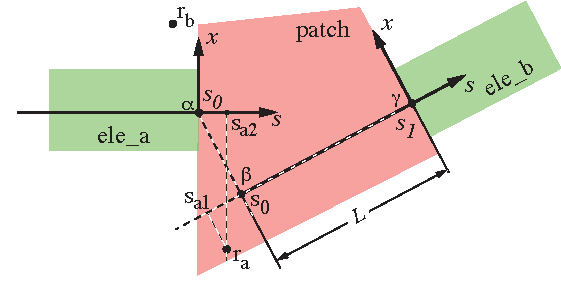
\includegraphics[width=5in]{patch-problem.pdf}
  \caption[The machine reference coordinates in a \vn{Patch} element.]
{The machine reference coordinates in a \vn{Patch} element. The \vn{Patch} element, shown
schematically as an irregular quadrilateral, is sandwiched between elements \vn{ele_a} and
\vn{ele_b}. \vn{L} is the length of the \vn{Patch}. In this example, the \vn{Patch} has a finite
\vn{y_rot}.}
  \label{f:patch.prob}
\end{figure}

%---------------------------------------------------------------------------------------------------
\section{Patch}
\label{s:patch}

A \vn{Patch} element shifts the reference orbit and time. Also see \vn{FloorShift}
(\sref{s:floorshift}) and \vn{Fiducial} (\sref{s:fiducial}) elements. A common application of a patch
is to orient two branch lines with respect to each other. 


A \vn{Patch} (\sref{s:patch}) element is different in that there is no ``natural'' coordinate 
system to use within the Patch. This is generally not an issue when the region inside the
Patch is field and aperture free since particle tracking can be done in one step from edge
to edge. However, when there are fields or apertures an internal
coordinate system is needed so that the fields or apertures can be unambiguously positioned.



%----
There 


Generally, if a particle is reasonably near the machine reference curve, there is a one-to-one mapping
between the particle's position and machine $(x, y, s)$ coordinates. 


with a non-zero \vn{x_rot} or non-zero \vn{y_rot} breaks the one-to-one mapping. This is
illustrated in \fig{f:patch.prob}.  The \vn{Patch} element, shown schematically as an, irregular
quadrilateral, is sandwiched between elements \vn{ele_a} and \vn{ele_b}. The machine coordinate system
with origin at $\alpha$ are the coordinates at the end of \vn{ele_a}. The coordinates at the end of
the \vn{Patch} has its origin labeled $\gamma$. By convention, the length of the patch \vn{L} is
taken to be the longitudinal distance from $\alpha$ to $\gamma$ with the \vn{Patch}'s exit
coordinates defining the longitudinal direction. The ``beginning'' point of the \vn{Patch} on the
reference curve a distance \vn{L} from point $\gamma$ is labeled $\beta$ in the figure.

In the machine $(x, y, s)$ coordinate system a particle at $\alpha$ will have some value $s = s_0$. A
particle at point $\beta$ will have the same value $s = s_0$ and a particle at $\gamma$ will have $s
= s_1 = s_0 + L$. A particle at point $r_a$ in \fig{f:patch.prob} illustrates the problem of
assigning $(x, y, s)$ coordinates to a given position. If the particle is considered to be within
the region of \vn{ele_a}, the particle's $s$ position will be $s_{a2}$ which is greater than the
value $s_0$ at the exit end of the element. This contradicts the expectation that particles within
\vn{ele_a} will have $s \le s_0$.  If, on the other hand, the particle is considered to be within
the \vn{Patch} region, the particle's $s$ position will be $s_{a1}$ which is less than the value
$s_0$ at the entrance to the patch. This contradicts the expectation that a particles within the
\vn{Patch} will have $s \ge s_0$.

To resolve this problem, \accellat considers a particle at position $r_a$ to be within the \vn{Patch}
region. This means that there is, in theory, no lower limit to the $s$-position that a particle in
the \vn{Patch} region can have. This also implies that there is a discontinuity in the $s$-position
of a particle crossing the exit face of \vn{ele1}. Typically, when particles are translated from the
exit face of one element to the exit face of the next, this \vn{Patch} problem does not appear. It
only appears when the track between faces is considered.

Notice that a particle at position $r_b$ in \fig{f:patch.prob} can simultaneously be considered to
be in either \vn{ele_a} or the \vn{Patch}. While this creates an ambiguity it does not complicate
tracking.

%---------------------------------------------------------------------------------------------------
\section{Quadrupole}
\label{s:quadrupole}

A \vn{Quadrupole} is a magnetic element with a linear field dependence
with transverse offset (\sref{s:mag.field}).


%---------------------------------------------------------------------------------------------------
\section{RFCavity}
\label{s:rfcavity}

An \vn{RFCavity} is an RF cavity without acceleration generally used in a storage ring. The main
difference between an \vn{RFCavity} and an \vn{LCavity} is that, unlike an \vn{Lcavity}, the
reference energy (\sref{s:phase.space}) through an \vn{RFCavity} is constant.

NOTE: This Element is in development and is incomplete.

%---------------------------------------------------------------------------------------------------
\section{Sextupole}
\label{s:sextupole}

A \vn{Sextupole} is a magnetic element with a quadratic field
dependence with transverse offset (\sref{s:mag.field}).


%---------------------------------------------------------------------------------------------------
\section{Solenoid}
\label{s:solenoid}

A \vn{solenoid} is an element with a longitudinal magnetic field.

%---------------------------------------------------------------------------------------------------
\section{Taylor}
\label{s:taylor}

A \vn{Taylor} element is a Taylor map (\sref{s:taylor.phys}) that maps the input orbital phase space and
possibly spin coordinates of a particle to the output orbital and
spin coordinates at the exit end of the element.

NOTE: This Element is in development and is incomplete.

%---------------------------------------------------------------------------------------------------
\section{ThickMultipole}
\label{s:thickmult}

A \vn{ThickMultipole} is a general non-zero length multipole element.

%---------------------------------------------------------------------------------------------------
\section{Undulator}
\label{s:undulator}

An \vn{Undulator} is and element with a periodic array of alternating bends.
Also see \vn{Wiggler} elements.

NOTE: This Element is in development and is incomplete.

%---------------------------------------------------------------------------------------------------
\section{UnionEle}
\label{s:unionele}

A \vn{UnionEle} is an element that contains a collection of other elements.
A \vn{UnionEle} is used when elements overlap spatially which happens with superposition (\sref{c:super}).

%---------------------------------------------------------------------------------------------------
\section{Wiggler}
\label{s:wiggler}

A \vn{Wiggler} is and element with a periodic array of alternating bends.
Also see \vn{Undulator} elements.

NOTE: This Element is in development and is incomplete.
